\documentclass{ctexart}

\usepackage{ctex}
\usepackage{subfigure}
\usepackage{CJK}
\usepackage{siunitx}
\usepackage{amsmath}
\usepackage{amssymb}
\usepackage{graphicx}
\usepackage{cite}
\usepackage{multirow}
\usepackage{float}
\usepackage{xltxtra}
\usepackage[a4paper,left=1.25in,right=1.25in,top=1in,bottom=1in]{geometry}
%标题, 作者

\title{Mandelbrot Set 的生成和探索}

\author{作者姓名: 唐浩 \\ 专业和学号: 信息与计算科学 3200102118}

\begin{document}

\maketitle

\renewcommand{\abstractname}{摘要} %摘要
\bibliographystyle{plain}

\begin{abstract}

  本文就 Mandelbrot Set \cite{1989The} 的生成进行探索,简要介绍一下 Mandelbrot Set 的起始,数学推导,后给出具体的程序说明,并附上一定的图片解释。通过计算机,我们可以进行相对于人脑来说较麻烦的计算,通过计算机进行迭代,我们可以简单重现 Mandelbrot Set 的生成过程。
  
\textbf{关键字:Mandelbrot Set 迭代 图形生成}

\end{abstract}

\section{引言} %引言

{\bf Mandelbrot Set} \cite{1998The} 曾被称为{\bf ``上帝的指纹'' ``魔鬼的聚合物''},它是由{\bf Benoit B. Mandelbrot}教授
\begin{figure}[H]
\centering
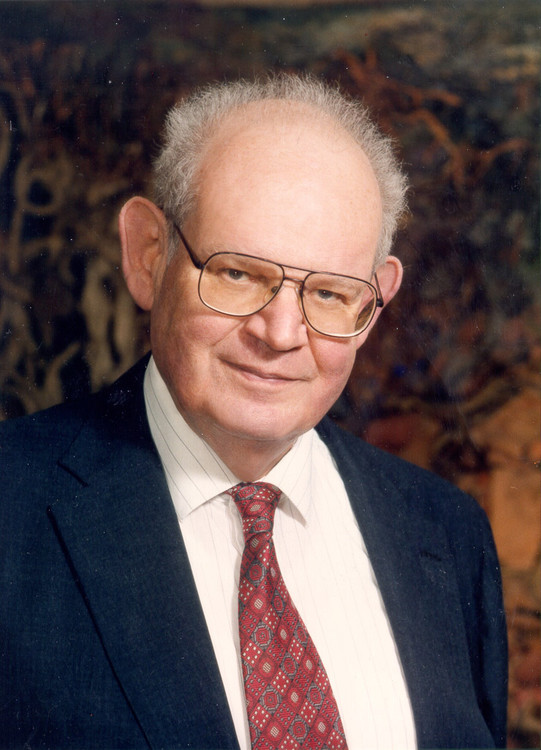
\includegraphics[scale=0.1]{mandelbrot.jpeg}
\end{figure}
在二十世纪七十年代发现的。它是一个几何图形,其中的点均出自迭代公式:{\bf $Z_{n+1} = Z_n^2 + C$},对于每一个C, 从$Z = 0 + 0i$开始计算,若$Z_n$收敛,则C在集合中。对于所有的C组成的集合,便称为{\bf Mandelbrot Set}。本文主要介绍如何生成 Mandelbrot Set,并就其各种格式进行一个初步的探索。主要通过去选取不同的参数,对生成的图进行解释,得出一定的结论。


%数学理论, 算法, 数值算例, 结论
\section{数学理论}
\subsection{迭代}

首先,我们来介绍一下什么是迭代。迭代是重复反馈过程的活动,其目的通常是为了逼近所需目标或结果。每一次对过程的重复称为一次“迭代”,而每一次迭代得到的结果会作为下一次迭代的初始值。就 Mandelbrot Set 而言,被迭代的是一些最简单的函数,其形如 $f(x) = x^2 + C$(C 为常量)。

对于每一个C,若根据迭代规则: $Z_{n+1} = Z_n^2 + C$ 生成的序列$\{x_0, x_1,\dots\} \rightarrow \infty$ ,则Z的轨迹无界,则 $C \notin$  Mandelbrot Set,若序列有界,则 $C \in$ Mandelbrot Set 。

\subsection{逃逸时间算法}
\subsubsection{逃逸法则}

对于一个复数 $z_n = x_n + y_ni$, 模 $|z_n| = \sqrt{x_n^2 + y_n^2}$ 。定义:

如果对于一个复数序列 $\{z_1, z_2, \dots, z_n\}$ 有 $|z_j| > max(2,|C|)$ 则序列将逃逸到无穷大。

\subsubsection{逃逸时间算法}

对于每个复参数平面上的点C,我们生成一个序列Z,根据逃逸准则,我们规定R为逃逸半径,在 $\{z_1, \dots z_n\}$ 里,如果 $|z_j| < R$ ,判断有界(但其实也有可能这个序列是无界的),反之,这个序列无界。故需要确定以下参数:

1、复平面范围 $C = \{c = x + yi: x_1 \le x \le x_2, y_1 \le y \le y_2 \}$
  
2、分辨率gridSize

3、逃逸半径 $R = max(2, |C|)$

4、逃逸时间 N = 最大迭代次数

\section{算法}
\begin{verbatim}
#include <iostream>
#include <cstdlib>
#include "Window.h"
#include "Manderbrot.h"
#include "bitmap.h"

int main(argc, *argv[])

if argc < 5
then cerr << "Usage: " << argv[0] << " filename ox oy dimension" << endl
exit(-1)

Window win(atof(argv[2]), atof(argv[3]),atof(argv[4]))

lpp <- win.get_lpp()
dim <- win.get_dimension()
width <- win.get_width()
height <- win.get_height()
ox <- win.get_ox() - dim
oy <- win.get_oy() - dim / width * height
N <- 100
*cache <- new char[width * height * 3]

for j <- 0 to height
for i <- 0 to width

x <- ox + lpp * i
y <- oy + lpp * j
pos <- width * j + i;
Manderbrot man(complex<double>{0.0, 0.0}, N, complex<double>{x, y})

while !man.stop_criterion()
man.forward_step()
if man.is_disconvergence()
then break

if man.stop_criterion()
then 
cache[pos * 3] <- 255
cache[pos * 3 + 1] <- 255
cache[pos * 3 + 2] <- 255
else
cache[pos * 3] <- 0
cache[pos * 3 + 1] <- 0
cache[pos * 3 + 2] <- 0
build_bmp(argv[1], width, height, cache)
delete [] cache

return 0
\end{verbatim}

\section{数值算例}

以下为原点在(0,0)时修改N所得到的不同图像:
\begin{figure}[H]
\centering
\subfigure[N = 10]
    {
        \centering
        \includegraphics[width=0.45\textwidth]{test.bmp}
    }
\subfigure[N = 20]
    {
        \centering
        \includegraphics[width=0.45\textwidth]{test1.bmp}
    }
\end{figure}

\begin{figure}[H]
\centering
\subfigure[N = 100]
    {
        \centering
        \includegraphics[width=0.45\textwidth]{test2.bmp}
    }
\subfigure[N = 10000]
    {
      \centering
      \includegraphics[width=0.45\textwidth]{test4.bmp}
    }
\end{figure}

下面我们将原点偏移,可以得到具体部位的一个放大图,以 N = 100 为例:
\begin{figure}[H]
\centering
\subfigure[原点:(0.0,1.0,1)]
    {
        \centering
        \includegraphics[width=0.45\textwidth]{test5.bmp}
    }
\subfigure[原点:(0.0,0.8,0.1)]
    {
        \centering
        \includegraphics[width=0.45\textwidth]{test6.bmp}
    }
\end{figure}

\section{结论}

Mandelbrot Set 的图形表示可以让我们认识到纯粹的数学之美,与之相关的分形几何学则是无处不在的,不得不感叹数学的力量。由于分形几何学知识的匮乏,本文只能给出Mandelbrot Set的定义,并以最容易理解的方式绘制出该集合。这里使用的语言是C++。我们还可以给 Mandelbrot Set添加不同的颜色,由于时间因素,就不进行颜色的添加了。 \cite{王伊蕾2015LaTeX}

\bibliographystyle{plain}
\bibliography{ckwx.bib}

\end{document}
